\documentclass[a4paper,10pt]{article}
\usepackage[french]{babel}
\usepackage[utf8]{inputenc}
\usepackage[top=2cm, bottom=2cm, left=2cm, right=2cm]{geometry}
\usepackage{setspace}
\usepackage[T1]{fontenc}
%\usepackage{listings}
\usepackage{graphicx}
\usepackage{color}
\usepackage[table, dvipsnames]{xcolor}
\usepackage{listings}
\usepackage{amsmath}
\usepackage{algorithmic}
\usepackage{amssymb}
\usepackage{lmodern}
\usepackage[french,boxed,ruled,lined]{algorithm2e}
\definecolor{darkWhite}{rgb}{1.00,1.00,1.00}
\xdefinecolor{red}{named}{Red}
\xdefinecolor{blue}{named}{Blue}
\xdefinecolor{orange}{named}{Orange}
\lstset{
aboveskip=4mm,
belowskip=0mm,
backgroundcolor=\color{darkWhite},
breakatwhitespace=false,
captionpos=b,
commentstyle=\color{red},
deletekeywords={...},
escapeinside={\%*}{*)},
extendedchars=true,
keepspaces=true,
literate=
{²}{{\textsuperscript{2}}}1
{⁴}{{\textsuperscript{4}}}1
{⁶}{{\textsuperscript{6}}}1
{⁸}{{\textsuperscript{8}}}1
{€}{{\euro{}}}1
{é}{{\'e}}1
{è}{{\`{e}}}1
{ê}{{\^{e}}}1
{ë}{{\¨{e}}}1
{É}{{\'{E}}}1
{Ê}{{\^{E}}}1
{û}{{\^{u}}}1
{ù}{{\`{u}}}1
{â}{{\^{a}}}1
{à}{{\`{a}}}1
{á}{{\'{a}}}1
{ã}{{\~{a}}}1
{Á}{{\'{A}}}1
{Â}{{\^{A}}}1
{Ã}{{\~{A}}}1
{ç}{{\c{c}}}1
{Ç}{{\c{C}}}1
{õ}{{\~{o}}}1
{ó}{{\'{o}}}1
{ô}{{\^{o}}}1
{Õ}{{\~{O}}}1
{Ó}{{\'{O}}}1
{Ô}{{\^{O}}}1
{î}{{\^{i}}}1
{Î}{{\^{I}}}1
{í}{{\'{i}}}1
{Í}{{\~{Í}}}1,
morekeywords={*,...},
numbers=left,
numbersep=10pt,
numberstyle=\tiny\color{black},
rulecolor=\color{black},
showspaces=false,
showtabs=false,
stepnumber=1,
tabsize=4,
title=\lstname,
showstringspaces=false,
basicstyle=\footnotesize\ttfamily,
keywordstyle=\bfseries\color{green!40!black},
identifierstyle=\color{blue},
stringstyle=\color{orange},
}


\begin{document}

\title{Projet S6 : Acting Shooting Star }
\author{Ibrahim LMOURID \& Houssam BAHHOU \& Ayoub LASRI \& Eloi MAGON De La VILLEHUCHET}


\label{sec:title}
\thispagestyle{empty}



\includegraphics[width=0.4\textwidth]{Logo.png}
\\
\\
\\
\\
\\
\noindent\rule{\textwidth}{1pt}
\begin{flushright}
  \Huge
  \textbf{Rapport de Projet }

    \vspace{15pt}
  \large 
  \textsl{Acting Shooting Star }

\end{flushright}
\noindent\rule{\textwidth}{1pt}

\vspace{\stretch{1}}

\large
\noindent\textbf{Auteurs   : }  \textup{Ibrahim LMOURID \& Houssam BAHHOU \& Ayoub LASRI \& Eloi MAGON De La VILLEHUCHET - Equipe $n^{o}$ 9152 } \\
\noindent\textbf{Encadrants :} \textup{ Madame Joséphine Calandra  }
\vspace{\stretch{1}}
\vspace{\stretch{0.5}}

\normalsize
\begin{center}
  Première année, Semestre 6,Filière informatique,ENSEIRB-MATMECA\\
  Date : \today
\end{center}

\vspace{\stretch{1}}


\newpage
\tableofcontents

\newpage
\section{Introduction}
Dans le cadre du semestre 6 de l'enseignement en formation d'ingénieur Informatique dispensée au sein de l'Enseirb-Matmeca, nous étions amenés à exploiter nos savoirs théoriques de l'UE-A ainsi que nos connaissances pratiques de l'UE-B, notamment celle liée à la programmation fonctionnelle, afin de réaliser ce projet.
\newline

Le groupe est composé de quatre membres :  Ibrahim LMOURID, Houssam BAHHOU, Ayoub LASRI, Eloi MAGON De La VILLEHUCHET.
\newline

Ce projet était encadré par Madame Joséphine CALANDRA mais nous avons aussi pu recevoir des conseils de la part de Monsieur David RENAULT, responsable des projets.

\section{Présentation du sujet}
\label{presentation}
\subsection{Description du projet}
Dans ce projet intitulé \textit{Acting Shooting Star} nous étions amenés à exploiter nos connaissances en programmation fonctionnelle afin de construire une bibliothèque d'acteurs permettant de créer un jeu du type \textit{shoot'em up} (jeu ou l'on dirige un véhicule ou un personnage devant détruire un grand nombre d'ennemis à l'aide d'armes). Ces acteurs interagirons entre eux par le biais de messages qu'ils auront la possibilité de s'envoyer et de recevoir. Ces messages permettent de :\\

\begin{itemize}
    \item Assurer la mise à jour de l'état des acteurs.\\
    \item Émettre d'autres messages.\\
    \item Créer de nouveaux acteurs.\\
    \item Tuer un ou plusieurs acteurs.\\
\end{itemize}
L'un des objectifs de ce projet, est de nous familiariser avec les concept de la programmation fonctionnelle.


Dans un premier temps, nous allons décrire les différentes structures nécessaires à la construction du jeux, ainsi que les fonctions de bases qui permettent de les manipuler. Ces structures permettent de donner une définition aux différents éléments du jeu, comme les acteurs et les messages.
\newline

Ensuite, nous allons présenter les différentes parties du projet telles que nous les avons conçues. Par conséquent, nous aurons l'occasion de décrire les différents algorithmes nécessaires au déroulement du jeux. 
\newline

D'une autre part, il est nécessaire de vérifier le bon fonctionnement de notre code, en s'assurant qu'il ne contient pas d'erreurs et qu'il respecte les exigence du sujet. Par conséquent, nous avons mis en places plusieurs tests de validation pour chaque partie de notre projet. Ces tests permettent de détecter les différentes erreurs, afin de les corriger au plus vite. 
\newline

Enfin, il est important d'analyser notre travail, ceci nous permettra de décrire les différentes limites de notre conception, ainsi que les améliorations que nous pourrions apporter.
%On utilise pour mener à bien ce projet la programmation fonctionnelle, et plus précisément le langage racket. 
 
\subsection{Problématique}

Les principales tâches ont été en premier lieu d'implémenter les structures qui permettront de représenter les acteurs, les messages qu'ils s'échangent mais aussi le monde dans lequel ils évoluent. Le second objectif est de réaliser un affichage de ces acteurs directement dans le terminal pour un rendu final ressemblant le plus possible à un jeu, même si le but final reste la bonne implémentation de la bibliothèque d'acteurs.

\subsection{Organisation du projet}
\subsubsection*{Langage de programmation}
L'un des objectifs de ce projet, est de nous familiariser avec les notions de la programmation fonctionnelle. Par conséquent, nos différents algorithmes sont implémentés en \textit{Racket}.
\subsubsection*{Répartition des tâches}
Le bon déroulement de notre travail, nécessite de déterminer les différentes tâches à réaliser afin de les répartir entre les différents membres du groupe.\\

Voici la liste des tâches qui ont aiguillé notre projet :\\
\begin{itemize}
    \item Définir des structures qui définissent les acteurs et les messages, ainsi que les fonctions de base qui permettent de manipuler ces structures.\\
    \item Écrire les fonctions qui permettent de gérer l'ensemble des acteurs sur un intervalle de temps.\\
    \item Utiliser la bibliothèque \textit{raart} pour gérer l'affichage des acteurs.\\
    \item Écrire le code qui permet de gérer les collisions entre les acteurs.\\
    \item Gérer l'animation par le biais de la bibliothèque \textit{Lux}.\\
    \item Écrire les fonctions qui permettent de remonter le     temps.\\
    \item Écrire la documentation afin de préciser le fonctionnement de notre code à un utilisateur externe.\\
    
\end{itemize}
Nous avons travaillé sur ses tâches en partageant nos avancées en temps réel, par le biais du logiciel de gestion de dépôt : \textit{Git}.

\subsection{Architecture du projet}

Les fichiers dans le dépôt sont organisés de la manière suivante :

\begin{center}
     \begin{verbatim}
        /               -- la racine du répertoire du projet
        README.md       -- fichier qui contient les instructions d'exécution
        Makefile        -- Makefile global
        /src            -- fichiers sources (.rkt/scrbl)
        /src/main.rkt   -- fichier principal
        /doc            -- fichiers de la documentation
        /rapport        -- rapport du projet (.tex/pdf)
    \end{verbatim}
\end{center}

\section{Explication des algorithmes et des implémentations choisies} 
\label{structfonc}
\subsection{Structures et fonctions de bases}
\label{structs}
Le sujet aborde un modèle de programmation concurrent, c'est le modèle \textbf{Acteur}, c'est un modèle mathématique qui considère, dans un monde, un ensemble des acteurs comme des fonctions primitives communiquant par échange de messages.\\
Ce modèle considère donc que tout est acteur (de la même manière qu’en programmation orienté objet, on considère que tout est objet) et qu’il doit être en mesure de :
\begin{itemize}
    \item Recevoir des messages
    \item Envoyer des messages à d’autres acteurs
    \item Créer de nouveaux acteurs
    \item Modifier son état (et donc potentiellement son comportement pour les messages suivants)
\end{itemize}
L'objectif donc du projet consiste à mettre en place une bibliothèque d'acteurs afin de permettre de construire un jeu ressemblant à \textbf{un shoot'em up},
Pour donner une représentation symbolique au modèle \textbf{Acteur} nous avons pensé à implémenter les deux structures suivantes qui justifient le principe de communication par messages entre les acteurs:
\subsubsection{Les structures actors et msg}
%% définir les deux struct & expliquer que les acteurs jouent dans un monde %%
\textbf{\texttt{La structure actor}} va englober tout les acteurs du jeux. Pour faire le parallèle avec un jeu de type shoot'em up: ces acteurs sont l'implémentation des différents éléments que l'on peut voir à l'écran : le vaisseau contrôlé par le joueur, des ennemis, des missiles etc ... 
\newline
On implémente donc la structure actors sous cette forme : 
        \begin{lstlisting}
        (struct actor (state mailbox location))
        \end{lstlisting}
Cette structure comporte 3 champs : \\
\begin{itemize}
    \item  le champ \textbf{'state'} correspond à l'état de l'acteur, c'est à dire s'il s'agit d'un \textbf{\texttt{shooter}}, d'un obstacle (\textbf{\texttt{Wall}}), d'une missile \textbf{\texttt{missile}}, etc... Cette structure aura notamment son importance lors de l'affichage, puisque selon leur états, les acteurs bénéficieront d'une représentation différente;\\
    \item le champ \textbf{'mailbox'} a pour rôle de stocker une liste de messages qui lui auront été envoyé par d'autres acteurs ou par l'utilisateur;\\
    \item le champ \textbf{'location'} contient les coordonnées de l'acteur.\\
\end{itemize} 
\hfill
\newline
\textbf{\texttt{La structure msg}} est l'implémentation des messages échangés par les acteurs. Ces messages sont chargés de transporter l’information d’un acteur à l’autre, ils contiendront des instructions que les acteurs exécuteront. En fait, Ils peuvent être de plusieurs types selon l'instruction qu'ils contienne : déplacer un acteur (\textbf{\texttt{move}}) , créer un nouvel acteurs (\textbf{\texttt{La structure msg}}), ...
        \begin{lstlisting}
        (struct msg (etiquette coord dest))
        \end{lstlisting}
Les champs de cette structure sont les suivants : \\
\begin{itemize}
    \item le champ \textbf{'étiquette'} est une chaine de caractère indiquant le type de message;\\
    \item le champ \textbf{'coord'} contient des coordonnées transmise à un acteur dans le cas d'un message de type "move" qui enjoint à un acteur de se deplacer à ladite coordonnée.\\
    \item le champ \textbf{'dest'} est une chaine de caractère qui permet d'indiquer à quel(s) acteur(s) s'adresse le message.\\
\end{itemize}
La figure (\ref{fig:act}) ci-dessous montre une représentation schématique du modèle acteur :

\begin{figure}[h]
\begin{center}
    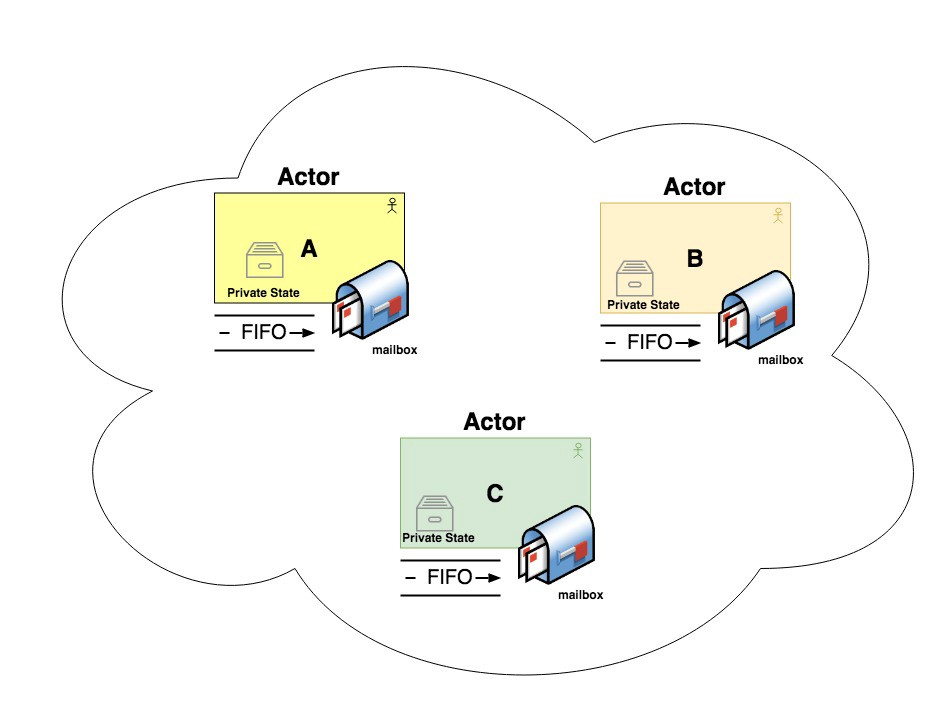
\includegraphics[scale=0.3]{actor.jpeg}
        \caption{Modèle Acteur}
    \label{fig:act}
\end{center}
\end{figure}

La politique choisie en terme d'envoi des messages est donc d'envoyer chaque messages à tous les acteurs, le champ destination permettra aux acteurs de choisir les messages qu'ils prendront en compte.
\subsubsection{Fonctions de bases}
\label{base}
Afin de manipuler les champs de ces structures, et permettre aux acteurs de communiquer entre eux, et de mettre à jour leurs états, il est nécessaire de se pencher sur des fonctions que nous avons écrites et utilisées pour permettre au jeu de fonctionner.
\begin{itemize}
\item \textbf{\texttt{actor-send}} : Les acteurs communiquent via des messages, la première étape est donc de créer une fonction \emph{actor-send} prenant un message et un acteur en argument qui renvoie un nouvel acteur ayant reçu le message dans sa mailbox.\\
\item \textbf{\texttt{move}} : La fonction \emph{move} renvoie simplement un message pourvu de l'étiquette 'move' et des coordonnées $x$ et $y$ passées en argument. Si un acteur reçoit ce message, il se déplace aux coordonnées indiquées au moment de la mise à jour des acteurs. \\
\item \textbf{\texttt{create-missile}}: qui permet de créer d'un acteur père, un acteur fils de type 'missile'.\\
Ces fonctions sont assez simple, et se font dans un temps constant.\\ 
\item \textbf{actor-update} : Nous avons vu que les acteurs possèdent un 'mailbox' pour stocker les messages reçues. A la fin de chaque intervalle de temps, ils vident leur 'mailbox' et se mettent à jour en fonction de ce qu'ils ont reçu. Il a également été précisé que chaque message était envoyé à tous les acteurs. Le rôle de cette fonction est donc d'une part de sélectionner les messages qui lui sont adressés et d'autre part de mettre à jour l'acteur selon ces messages. Il nous fallait donc écrire une fonction \emph{actor-update}, qui lors de son appel, va lire progressivement les messages contenus dans la mailbox, mettre à jour l'acteur selon l'instruction qui lui est envoyée et supprimer le message de la liste, cela jusqu'à ce que la liste soit vide. On utilise pour cela l'instruction \texttt{letrec}.\\
Rappelons qu'un Acteur est une file d’attente (mailbox), un état, un comportement, un statut et aussi un ensemble d’Acteurs enfants. Ce qui nous oblige d'adapter la fonction \textbf{actor-update} pour permettre à l'acteur d'envoyer des messages à d'autres acteurs, ainsi que de créer d'autres acteurs fils.\\
L'idée c'est de programmer cette fonction  de manière à ce qu'elle renvoie deux listes, une liste des acteurs enfants (exemple d'un \textbf{\texttt{shooter}} qui lance une \textbf{\texttt{missile}}), ainsi qu'une liste des messages.\\
Cette fonction a \textbf{une complexité linéaire} par rapport à la taille du mailbox.
\end{itemize}
\hfill
\newline
Notre objectif maintenant est de traiter l'ensemble des acteurs d'une manière assez générale, cela nous mène à penser à une structure de données globale servant de \textbf{runtime} organisant la mise à jour simultanée de tous les acteurs.\\
Pour cela il faut d'abord construire \textbf{une structure World} rassemblant l'ensemble des acteurs.
\subsubsection{La structure world}
Nos besoins ayant évolués au gré de l'avancement du projet, la structure 'world' a connu plusieurs implémentations successives. Son but est de représenter le monde dans lequel les acteurs évoluent, elle joue un rôle majeur dans l'affichage de la bibliothèque d'acteur. On présente ici la dernière implémentation que nous avons retenu : 

        \begin{lstlisting}
        (struct world (actors states depth tick))
        \end{lstlisting}
Voici le rôle de ses quatre champs: \\
\begin{itemize}
    \item Le champ \textbf{actors} est la liste de tous les acteurs présent dans le monde; \\
    \item Le champ \textbf{states} correspond à une liste des états antérieur du monde, ils permettent d'effectuer la remontée dans le temps. \\
    \item Le champ \textbf{depth} est un entier qui correspond au nombre d'état duquel on est remonté. \\
    \item Le champ \textbf{tick}, un nombre entier, représente l'évolution du monde avec le temps: A chaque tick des actions sont effectués par les acteurs, des messages sont échangés, et un nouveau monde est créé prenant en compte ces changements.\\
\end{itemize}
Ce type de donnée possède ainsi certaines méthodes permettant la manipulation de tout acteurs:\\
\begin{itemize}
    \item \textbf{world-send} : cette fonction permet d'envoyer un message à tous les acteurs du monde. Elle prend donc en argument le monde en question et un message et retourne un nouveau monde dans lequel le message à été ajouté à la mailbox de chaque acteur. On utilise ici un \textit{letrec} pour créer le nouveau monde en ajoutant progressivement le message à chaque acteur en utilisant la fonction actor-send décrite dans la section \ref{base}. Cette fonction a une compléxité linéaire par rapport au nombre des acteurs. \\
    \item \textbf{update-world} : cette méthode met à jour l'intégralité des acteurs du monde. Son fonctionnement est le même que la fonction world-send, en utilisant cette fois ci la fonction actor-update sur chaque acteur. Elle a une complexité en temps $O(n \times m)$ avec n est le nombre des acteurs et m est la taille du 'mailbox' de chaque acteur. \\
\end{itemize}
La définition de la structure est en réalité plus complexe et contient de nombreuses autres informations. Celles-ci sont lié à l'utilisation de lux, est seront donc décrite dans la section \ref{affichage}.


%% actor-send / move / update / collision / kill %%

%% idée partie de collision2 et essayer de détailler une execution de collision2 en remplacant les fonctions qui y sont call%%


\subsection{Déroulement du jeu}
\label{deroule}
\subsubsection{La bibliothèque \emph{Lux} et gestion du jeu}
Une fois les fonctions régissant les interactions basiques entre acteurs implémentées, il est nécessaire d'animer le monde afin de mettre en place le jeu en lui même. \\
On introduit ainsi la bibliothèque \emph{Lux} qui permet de créer une structure représentant l’état global de la structure \textbf{World}, en effet \emph{Lux} donne la possibilité de représenter l’évolution des acteurs au cours du temps, et d’autre part elle permet à l’utilisateur de donner des instructions à certains acteurs en appuyant sur des touches de son clavier.\\
Cette dernière ajoute dans la définition de la structure \textbf{World} un certain nombre de fonctions dont allons détailler l'utilité  : \\
\begin{itemize}
    \item \textbf{world-fps} : Cette fonction permet de choisir le nombre d'image par seconde affiché lors de l'animation; \\
    \item \textbf{world-label} Renvoie le titre de la fenêtre contenant l'application; \\
    \item \textbf{world-event} Permet de renvoyer un nouvel état du monde à partir d'un évènement. Ces évènements correspondent ici à la pression exercée sur une touche par l'utilisateur, selon la touche appuyée, on décide dans cette fonction de quelle façon le monde va être modifié; \\
    \item \textbf{world-output} affiche l'état du monde, ici, on renvoie simplement le résultat de la fonction \textit{display-world} décrite prochainement dans la partie \ref{aff}; \\
    \item \textbf{world-tick} Cette fonction renvoie un nouveau monde à chaque tick d'horloge à partir du monde précédent. On détaille ci-après son fonctionnement de manière plus précise. \\
\end{itemize}
\subsubsection{Gestion de collision}
\begin{itemize}
\item La gestion de collision entre acteur est une partie essentielle dans l'implémentation du jeu, afin de réaliser cette tache  plusieurs fonctions sont concernées : \\
\begin{itemize}
    \item La fonction \textbf{\texttt{actor-collision?}} qui pour deux acteurs passés en argument renvoie le booléen Vrai si les deux acteurs sont en collisions et Faux sinon. Deux acteurs sont considérés en collision s'ils ont les mêmes coordonnées. On a pris garde qu'un acteur ne puisse pas entrer en collision avec lui  même. \\
    \item \textbf{\texttt{collision1}} qui pour deux acteurs  et la liste d'acteurs du monde auquel ils appartiennent donnés en arguments, supprime le deuxième acteur si ceux-ci sont en collision.\\
    \item \textbf{collision-world} : son but est de supprimer tous les acteurs du monde en collision avec un acteur donné. La fonction prends en argument une liste d'acteur et un acteur. On utilise ici une stratégie récursive pour tester la collision avec chaque acteur de la liste. Elle fait appelle à la fonction auxiliaire \texttt{collision1}.
    \item Finalement la fonction \textbf{collision2} prends en argument une liste d'acteur et supprime de cette liste tous les acteurs qui sont en collisions.\\
\end{itemize}
\end{itemize}
Le pseudo-algorithme suivant résume le processus décrit précédemment:\\   
\begin{algorithm}
\caption{collision-world}
\begin{algorithmic}
\STATE actors\_list is the list of actors in the world and n it's length 
\IF{ Is\_Empty(actors\_list)}
\RETURN actors
\ENDIF
\FOR{actor1 in actors\_list}
    \STATE L2=remove actor from actor\_list
    \FOR{actor2 in L2}
        \STATE collision1(actor1, actor2, actors\_list)
    \ENDFOR
\ENDFOR
\end{algorithmic}
\end{algorithm}

La complexité de cet algorithme est $O(n^2)$ avec n est le nombre d'acteurs.
\subsubsection{Word-tick}
Comme indiqué précédemment cette fonction permet de  renvoyer un nouvel état du monde à chaque \textbf{tick}, en suivant le processus suivant : 
\begin{itemize}
    \item D'abord Cette fonction vérifie si notre joueur principale \textbf{"shooter"} est mort ou non, car cela implique la fin du jeu.
    \item Ensuite elle envoie au début de \textbf{tick} un message à tous les acteurs
    \item Après, elle met à jour les acteurs du World par la fonction \texttt{update-world}
    \item Enfin elle gère l'ensemble des collisions et bordures et renvoie le nouveau état du monde, avec un \textbf{tick} incrémenté de 1. 
\end{itemize}

\subsection{Fonctionnement du jeu}
\label{affichage}

Pour représenter l'évolution de notre bibliothèque d'acteur et leur évolution, il nous fallait mettre au point un affichage sur le terminal. Nous avons pour ce faire utilisé les bibliothèques \textit{Raart} et \textit{Lux}.
\subsubsection{Affichage}
\label{aff}
L'affichage à proprement parler est géré par la bibliothèque \textit{Raart}: Celle ci permet d'afficher des caractères de la table ASCII sur un terminal, dans différentes couleurs. Nous avons donc choisi quelle apparence nous voulions donner aux différents acteurs :\\ 
\begin{itemize}
    \item \textbf{Le vaisseau ou shooter} : est représenté par le caractère suivant : {\textcolor{Blue}{>}} \\
    \item \textbf{Les adversaires} : sont représentés par le caractère suivant: {\textcolor{Red}{<}} \\
    \item \textbf{Les murs}: sont représenté par la chaîne de caractère suivante : \textcolor{Red}{|\ |} \\
    \item \textbf{les missiles}: sont représentés par les caractères suivants, suivant qu'ils soient tirés par le joueur ou par un adversaire :  : \large{\textcolor{Orange}{\ -}} \ \ \ \small{\textcolor{Orange}{$\bigstar$}}  
\end{itemize}
\hfill
\newline

L'affichage d'un acteur dépendra donc du champ 'coordonnée' dont nous l'avions pourvu lors de sa définition. Pour \textit{Raart}, ces coordonnées correspondent aux coordonnées du plan formé par les colonnes et les lignes du terminal. Nous avons choisi de restreindre les positions du jeu à un cadre rectangulaire de dimension : $90 \times 20$ \\
%\newpage
Une fois ces choix effectués, nous avons écrit une fonction permettant de représenter tous les acteurs d'un monde, c'est la fonction \textit{display-world} cette fonction prend en argument une structure 'world' et affiche tous les acteurs de cette structure selon leur coordonnées. En plus des acteurs, cette fonction affiche également les bordures, le score, le titre du jeu et l'indication TIME TRAVEL si une remontée dans le temps est en cours.

La Figure \ref{affterm} montre le résultat que nous avons obtenu.
\newline

\begin{figure}[h]
\begin{center}
    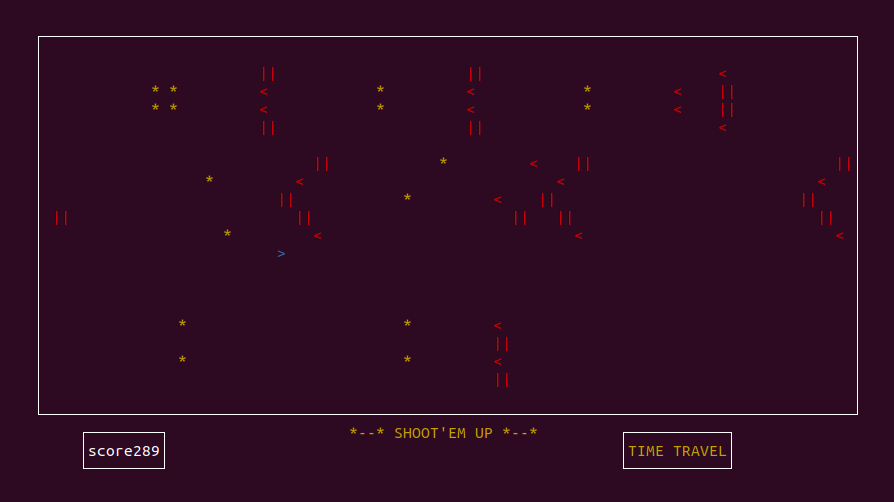
\includegraphics[scale=0.45]{affichage.png}
        \caption{Affichage de tous les acteurs sur un terminal}
    \label{affterm}
\end{center}
\end{figure}

\newpage
Sont également présentés en figures \ref{menu} et \ref{gameover} l'affichage d'un menu au démarrage du jeu et d'un message de 'game over' en cas de collision entre l'acteur principal et un autre acteur : 
\hfill
\newline
\begin{figure}[h]
\begin{center}
    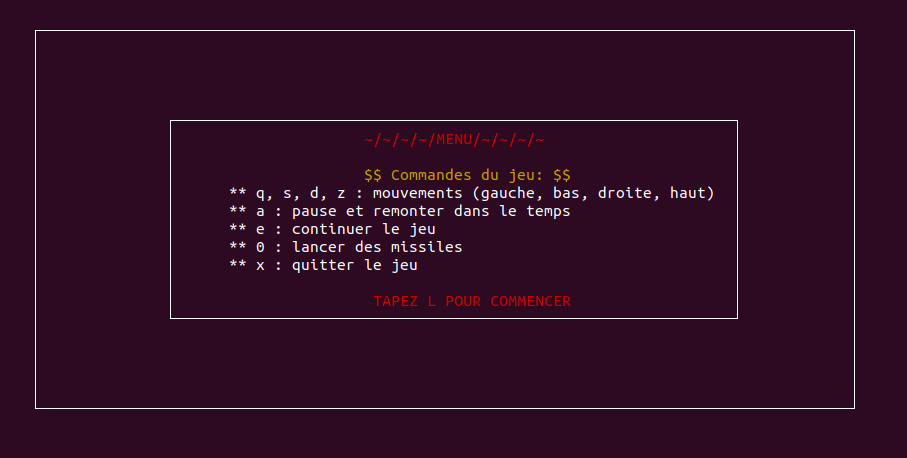
\includegraphics[scale=0.5]{menu.png}%
        \caption{Menu au lancement du jeu}
    \label{menu}
\end{center}
\end{figure}
  \hfill
\begin{figure}[h]
\begin{center}
    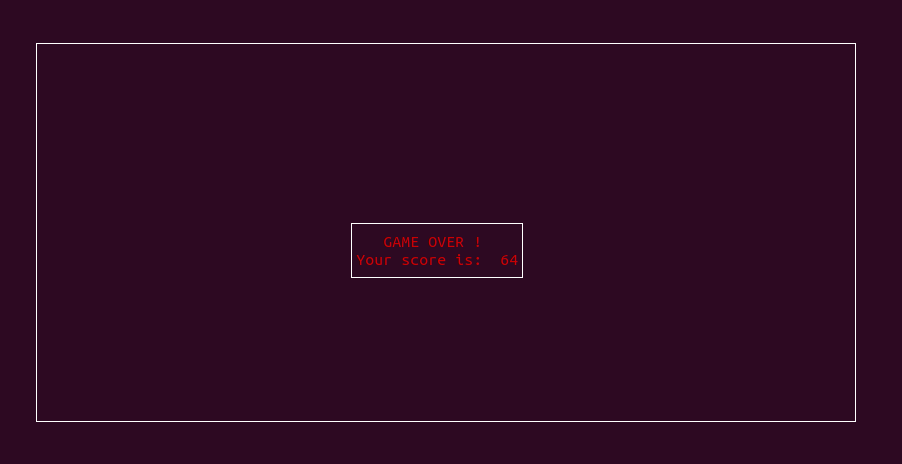
\includegraphics[scale=0.5]{game-over.png}
        \caption{Affichage de l'écran de Game Over}
    \label{gameover}
\end{center}    
\end{figure}
\newpage

\subsubsection{Contrôle du jeu par évènements}
Les différents évènements traités par la fonction \texttt{word-event} correspondent aux contrôles du jeu que l'on décrit ici : \\

Dans l'implémentation de notre bibliothèque d'acteurs, l'utilisateur contrôle un seul d'entre eux par l'intermédiaire des touches de son clavier. Il s'agit de l'acteur labellisé \textbf{shooter}. Voici les différents contrôles disponibles : \\
\begin{itemize}
    \item Les touches \textbf{q, d, z, s} permettent respectivement de déplacer l'acteur sur le gauche, la droite, vers le haut et le bas; \\
    \item les touches \textbf{a} et \textbf{e} gère la remontée dans le temps : une pression sur \textbf{a} 'freeze' le jeu et fais revenir tous les acteurs d'un tick dans le passé. La touche \textbf{e} permet de relancer le jeu; \\
    \item la touche \textbf{q} permet de quitter le jeu;\\
    \item la touche \textbf{l} permet de lancer le jeu, dans le cas où l'utilisateur se trouve dans le menu. \\
\end{itemize}
\hfill
\newline

\subsubsection{Remontée dans le temps}
Le sujet demandait en dernier lieu d'implémenter un moyen de remonter dans le temps, c'est à dire, de pouvoir afficher un certain nombre d'états antérieur à l'état courant. C'est la raison d'être des champs \textbf{states} et \textbf{depth} dans la structure world. On les utilise comme suit : 
Tout d'abord le champ state : cette liste contient n états antérieurs. Le nombre n est décidé à l'initialisation du monde avant le lancement du jeu. À chaque tick, la fonction word-tick en renvoyant le nouveau monde, ajoute le dernier état au champ state et supprime le premier, on conserve ainsi le même nombre d'états stockés, pour limiter la complexité spatiale.
Lorsque la remontée dans le temps est enclenchée, c'est à dire la touche 'a' pressée, la première chose est d'arrêter l'incrémentation des tick, word-event renvoie pour nouveau monde donc le premier état stocké dans la liste en décrémentant le champ depth (initialisé à $n$ avec $n$ le nombre d'états stockés dans states), mais sans incrémenter les ticks. En répétant l'opération, on peut ainsi remonter de n ticks. Pour relancer le jeu, il faut appuyer sur la touche 'e', la fonction word-event renvoie alors le monde sans le changer, mais en incrémentant les ticks, ce qui relance l'animation. On peut  aussi attendre d'avoir épuisé le nombre d'état disponible dans states, c'est à dire quand depth vaut 0, auquel cas, le jeu se relance immédiatement. 


\section{Tests, Contrats et Documentation}
\label{doc}
\subsection{La documentation}
Comme nous l'avons précisé au début de ce rapport, notre objectif est de construire une bibliothèque qui permet de créer un monde d'acteurs pouvant interagir entre eux. Par conséquent, il est nécessaire, qu'une personne externe puisse comprendre le fonctionnement de notre code. C'est pourquoi nous avons rédigé une documentation qui explique le rôle de chaque fonction dans notre code. Cette documentation a été rédigée par l'outil \textit{Scribble}. Les fichiers d'extension \textit{.scrbl}, peuvent se transformer en format documentation, de plusieurs types (pdf, html, \LaTeX ...) par le biais de la commande suivante : \\
\begin{center}
    \textit{scribble --dest doc actors\_documentation.scrbl} \\
\end{center}
Nous avons choisis de diviser notre documentation en deux grandes parties : \\
\begin{itemize}
    \item \textbf{Gestion des acteurs} : Dans cette partie nous avons expliqué la façon avec laquelle nous avons défini les acteurs et leurs interaction, ainsi que les prototypes et le rôle des fonctions de base qui permettent de les gérer. \\
    \item \textbf{Gestion du jeu} : Dans cette partie, nous avons présenté les les prototype et le fonctionnement de chaque fonction qui permet de gérer le jeu, son affichage ainsi que son animation. \\
\end{itemize}

Cette partition permet à chaque utilisateur externe de comprendre notre code tel que nous l'avons conçues.

\subsection{Contrats}
\label{contrats}
Au fil de notre projet nous avons créé un grand nombre de fonctions, ces dernières se doivent de prendre un certain type d'argument uniquement. Pour éviter les erreurs mais aussi pour mieux les comprendre nous avons créé un fichier de contrats (\textit{contracts.rkt}). Le but de ces contrats est de prendre pour chaque fonction un ensemble de prédicats que l’on peut passer sur
les paramètres d’entrée et de sortie des fonctions.\\
\\Nous avons tout d'abord implémenter les différentes fonctions permettant la définition des prédicats sur tout les champs des structures. Par exemple pour la structure actor nous avons défini 3 fonctions pour les trois champs location, state et mailbox sous la forme de 3 fonctions location?, state? et mailbox? renvoyant respectivement vrai ou faux si leur argument correspond au champ attendu.\\
\\Par la suite nous avons utilisé ces fonctions afin de créer des fonctions permettant de tester si un élément appartient bien à la structure en question.
En reprenant l'exemple de la structure actor nous avons implémenter la fonction actor? se basant sur les trois fonctions précédentes et permettant de tester si un élément appartient bien à la structure en question. \\
\\En utilisant cet ensemble de fonction et le système de contrat que nous fourni Racket nous avons mis en place des contrats sur un ensemble de fonction que nous avons utilisé au tout au long du projet. Ainsi, toute erreur sur le type d'argument lors de l'application d'une fonction était obligatoirement reconnue et déclarée.

\subsection{Description des tests de validation}
\label{tests}
Afin de nous assuré du bon fonctionnement de notre code nous avons créé des tests sur nos fonctions de bases qui ont été utilisé tout au long du projet. Nous avons défini une série de tests dans le fichiers \textit{tests.rkt,} à l'exécution de ce fichier l'ensemble des tests est parcouru, le nombre de test passé et le nombre d'échec est alors affiché. Pour chaque fonction que nous voulions tester nous avons mis en place plusieurs pour différents cas qui balayent les différents possibilités d'arguments pour chacune de ces fonctions afin de nous assurer qu'aucun n'ai été oublié lors de l'implémentions. Pour ce faire nous avons comparé les résultats obtenu par les fonctions aux résultats que nous attendions.
Afin d'assurer le déroulement du jeu nous avons veillé à tester particulièrement les fonctions de bases qui seront utilisés à de nombreuses reprises.\\
\\
L'ensemble du jeu repose sur les mouvements des acteurs et donc de l'envoi de message et de la lecture de la mailbox nous avons donc tester :
Les fonctions actor-send et actor-update et vérifier dans différents cas que l'acteur mis en argument de la fonction send reçoit bien le message que l'on veut lui délivrer et par la suite qu'il le prend bien en compte et met a jour sa position lorsque l'on exécute la fonction actor-update en le mettant en argument.\\
Notre bibliothèque permet de détecter les collisions, en effet au cours du jeu si deux acteurs se rencontrent, c'est à dire si ils ont les même position à un instant t ils doivent être supprimé. Nous avons donc vérifier que les fonctions qui permettent la suppression en cas de collision fonctionnait correctement.\\
\\
Ces tests associés aux contrats permettent facilement de détecter les erreurs dans nos fonctions. En effet à l'exécution de nos tests les arguments ne respectant pas les prédicats déclarés dans le fichier \textit{contracts.rkt} génèrent une erreur ce qui nous a permis d'avancer plus rapidement de la correction de notre code et les erreurs des tests eux même nous indique nos fautes dans l'implémentation.

\section{Discussion}
\subsection{Problèmes rencontrés}

\subsubsection{Problèmes liés à l'organisation}
Compte tenu de la situation sanitaire en France, liée à la pandémie du Covid-19, nous étions obligé à travailler ce projet en télétravail. Cette expérience était à la fois difficile et enrichissante. En effet, il était bien plus difficile d’échanger et de communiquer sur le projet et sur nos différents programmes, vu que nous n'avions pas la possibilité de se voir. Par conséquent, nous avons crée un groupe \textit{Facebook} pour pouvoir échanger. Cependant, les échanges par écrit sont souvent lents, c'est pourquoi nous avons décidé de discuter nos différent programmes sur \textit{Discord}. Cette plateforme, offre la possibilité de partager son écran avec les autres, ce qui est bien pratique pour discuter et expliquer son travail aux autres membres du groupes. Nous avons aussi décidé de mettre un maximum de commentaires à côté de chaque fonction pour permettre à chaque membres du groupe de comprendre le travail des autres.
\newline

Nous avons aussi utilisé la plateforme \textit{Slack}, pour échanger avec notre encadrante Madame Joséphine Calandra, ainsi que notre responsable de projet Monsieur David Renault.
\newline

Cette situation particulière a mis en valeur l'importance du logiciel de gestion de dépôts \textit{Git}, vu qu'il nous permettait de communiquer nos avancées en temps réel.
\subsubsection{Problèmes liés au codage de la bibliothèque}

L'une des principales difficultés que nous avons rencontré dans ce projet, était l'utilisation de la programmation fonctionnelle. En effet, depuis que nous avons commencé à apprendre à coder, nous avons utilisé principalement les notions de la programmation impérative. Ce projet, était donc l'occasion de nous familiariser avec les principes de la programmation fonctionnelle, ainsi que l'utilisation du langage de programmation \textit{Racket}. De plus, il nous a montré l'efficacité de ce mode de programmation, car il permet d'éviter plusieurs désagréments, comme la gestion manuelle de la mémoire, ainsi que les erreurs liées aux effet de bord.

En plus, nous étions parfois obligé à apporter des modifications à notre code pour le rendre compatible avec l'étape suivante.
\newline

En effet, avec les règles ajoutées par chaque nouvelle étape, nous devions revoir une partie de nos structures et de nos fonctions afin de les adapter aux nouvelles contraintes. Par exemple, nous avons modifié une bonne partie de notre code, pour qu'il prenne en considération les collisions entre les acteurs. Nous avons aussi rajouté des champs aux structures qui définissent les acteurs et les messages. Ceci nous a permis d'une part de créer des acteurs différents selon leur état (acteur principal, missile ...) et d'une autre part, de choisir les destinataires des messages envoyés par l'acteur, ceci lui permet d'envoyer une missile à un acteur de son choix. Nous avons même abandonner la structure \textit{world}, qui définit le monde des acteurs, pour la remplacer par la structure \textit{world} de la bibliothèque \textit{Lux}. Ceci nous a permis faciliter la gestion de l'animation du jeu.
\newline


Cependant, ces modification était enrichissantes, car elles nous ont permis de prendre du recul par rapport à notre travail, ce qui nous a permis d'améliorer notre code à chaque étape.


\subsection{Limites et améliorations possibles}

Les discussion entre les différents membres de l'équipe, ont montré qu'il est encore possible d'améliorer le jeu, pour qu'il devient plus difficile et plus amusant. Voici une liste de propositions qui permettent de réaliser cet objectif :\\


\begin{itemize}
    \item Dans notre bibliothèque d'acteurs, les ennemis se déplace de la droite vers la gauche. Il est possible d'augmenter la difficulté en permettant à ces acteurs d'avoir des sens, ou même des directions différentes. Cette modification nécessite aussi de donner à l'acteur principal la possibilité de choisir le sens de ses missiles. \\
    
    %\item Dans notre code, l'acteur principal a la possibilité d'envoyer des missiles à ces ennemis. Il peut être intéressant de donner aux autres acteurs la possibilité d'envoyer des missiles.\\
    
    \item Notre bibliothèque permet à l'acteur principal de tuer un seul ennemi par le biais d'un missile. Nous pouvons aussi créer un acteur "bonus" qui en cas de collision avec l'acteur principal, permet de tuer tous ses ennemis.\\
    
    \item Il est possible d'améliorer le jeu en ajoutant des niveaux de difficulté croissante. En effet, nous pouvons à chaque niveau, augmenter le nombre des ennemis. Nous pouvons aussi leur donner de nouveaux pouvoirs, ou bien augmenter leur vitesse.\\
    
    \item Nous pouvons donner à notre acteur principal un certain nombre de vies, afin de lui permettre de jouer plus longtemps.\\
    
    \item Nous pouvons utiliser le score de l'acteur principal afin de débloquer quelques bonus, augmenter la difficulté, passer à un niveau supérieur ou même terminer le jeu.\\
    
    %\item Il est aussi possible de rajouter un événement qui permet d'expliquer au joueur les règles ainsi que les touches qu'il faut utiliser.\\ 
    
    \item Nous pouvons rajouter un événement qui permet de lancer une nouvelle partie après avoir perdu.\\
    
    
\end{itemize}
%On peut ameliorer la doc



%\section{Méthodes mises en place}
%\subsection{Langage de programmation}
%\subsection{Gestion des dépôts}
%\subsection{Rédaction du rapport}

\section{Conclusion}
Ce projet a permis à l'ensemble des membres du groupe de s'épanouir et d'acquérir de nouvelles compétences. C'était aussi l'occasion de mieux comprendre les notions de la programmation fonctionnelle. Nous avons aussi réussi à nous familiariser avec le langage de programmation \textit{Racket}, ainsi que les différentes bibliothèque qu'il contient comme les bibliothèques que nous avons utilisé pour la gestion de l'affichage et l'animation du jeu \textit{Raart} et \textit{Lux}.
\newline

De plus, il nous a permis d'apprendre à gérer le travail en groupe, même dans cette situation particulière où nous devons travailler à distance  compte tenu des mesures de confinement, liées à la pandémie du Covid19. Les différentes discussions entre les membre de l'équipe furent constructives puisque composées de quatre pointe de vues différents.
\newline

Nous tenons à remercier notre encadrante Madame Joséphine Calandra, ainsi que notre responsable de projet Monsieur David Renault pour toute l'aide qu'ils nous ont apporté.

\section{Références}
https ://www.labri.fr/perso/renault/working/teaching/projets/
\\
\indent https ://thor.enseirb-matmeca.fr/
\\
\indent https://docs.racket-lang.org/
\\
\indent https://www.labri.fr/perso/renault/working/teaching/schemeprog/schemeprog.php
\end{document}
